\documentclass[tikz,border=8pt]{standalone}
% Shared look for every TikZ diagram. Load with \input{../../tools/tikz-style.tex}
\usepackage[T1]{fontenc}
\usepackage{lmodern}
\renewcommand{\sfdefault}{lmr}  % diagrams use the same serif as the text
\usetikzlibrary{arrows.meta, positioning, shapes.geometric, calc, fit, backgrounds}
\definecolor{cblue}{HTML}{4C78A8}
\definecolor{corange}{HTML}{F58518}
\definecolor{cgreen}{HTML}{54A24B}
\definecolor{cred}{HTML}{E45756}
\definecolor{cpurple}{HTML}{B279A2}
\definecolor{cgrey}{HTML}{6B6B6B}
\tikzset{
  every picture/.style={font=\sffamily, line width=1.2pt},
  box/.style={draw=#1, fill=#1!12, rounded corners=4pt, align=center, inner sep=7pt, minimum height=1.1cm},
  box/.default=cgrey,
  arrow/.style={-{Stealth[length=3mm]}, draw=cgrey, line width=1.4pt},
  title/.style={font=\sffamily\bfseries\Large},
  note/.style={font=\sffamily\small, text=cgrey, align=center},
}
\AtBeginDocument{\hyphenpenalty=10000 \exhyphenpenalty=10000}

\begin{document}
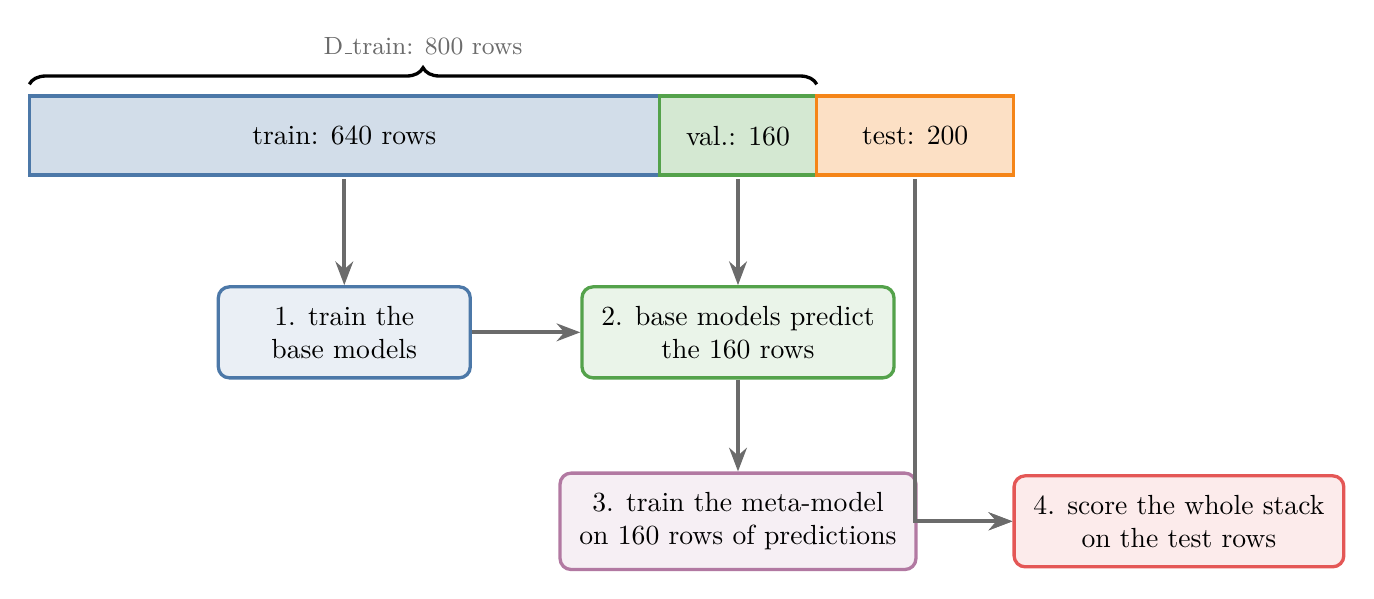
\begin{tikzpicture}[m/.style={box=cblue, minimum width=3.2cm}, k/.style={box=cpurple, minimum width=3.2cm}]
  % the data bar
  \fill[cblue!25, draw=cblue] (0,0) rectangle (8,1);
  \fill[cgreen!25, draw=cgreen] (8,0) rectangle (10,1);
  \fill[corange!25, draw=corange] (10,0) rectangle (12.5,1);
  \node at (4,0.5) {train: 640 rows};
  \node at (9,0.5) {val.: 160};
  \node at (11.25,0.5) {test: 200};
  \draw[decorate, decoration={brace, amplitude=6pt}] (0,1.15) -- node[above=7pt, note]{D\_train: 800 rows} (10,1.15);
  \node[m] (base) at (4,-2.0) {1. train the\\base models};
  \node[box=cgreen, minimum width=3.2cm] (pred) at (9,-2.0) {2. base models predict\\the 160 rows};
  \node[k] (meta) at (9,-4.4) {3. train the meta-model\\on 160 rows of predictions};
  \node[box=cred, minimum width=3.2cm] (score) at (14.6,-4.4) {4. score the whole stack\\on the test rows};
  \draw[arrow] (4,-0.05) -- (base); \draw[arrow] (9,-0.05) -- (pred);
  \draw[arrow] (base) -- (pred); \draw[arrow] (pred) -- (meta); \draw[arrow] (meta) -- (score);
  \draw[arrow] (11.25,-0.05) |- (score);
\end{tikzpicture}
\end{document}
